\setcounter{chapter}{1}
\chapter*{First year report}
\chaptermark{Chapter1}
\section{Introduction}
This analysis is aimed at measuring the CKM $\gamma$ angle using the tree-level decay \BToDK.\\
Despite many efforts from collaboration like \babar, \belle and \lhcb $\gamma$ is still the least constrained angle of the unitary triangle. Furthermore a precise measurement of $\gamma$ both through tree-level processes and loop mediated processes enables a possible discovery of New Physics (NP). This is particularly interesting since $\gamma$ is the only source of direct \CP violation in the Standard Model (SM) and current measurements of $\gamma$ can not account for the total \CP asymmetry observable in the universe. Searches for NP particularly for \CP violation mechanisms are essential.\\
\\
This analysis implements a model-independent approach to measuring $\gamma$. This means that the phasespace dependant \D meson decay amplitudes are evaluated such that direct measurements of related quantities are taken instead of using an amplitude model. This reduces a high systematic uncertainty on these amplitude models.\\
\\
Unless otherwise stated all activities described in this report were performed by the author.\\

\section{Theory overview}
\begin{figure}[!h]
\vspace*{-0.cm}
  \begin{center}
 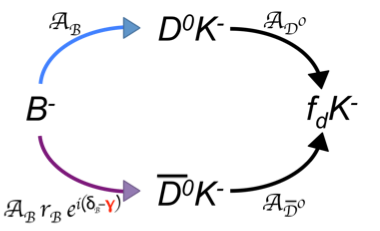
\includegraphics[width=0.49\textwidth]{interfere.png}
  \vspace*{-0.5cm}
  \end{center}
  \caption{\textit{Interfering decay paths for the $\Bm \rightarrow f_{\D} \Km $ decay. The $\gamma$ angle enters in the $\bquark \rightarrow \uquark $ transition.}}
  \label{fig:amp}
\end{figure}
In order to measure $\gamma$ the interference between the decay paths shown in Figure \ref{fig:amp} is used. This technique works only for processes where the \D meson final states is accessible to both \Dz and \Dzb mesons. The partial decay width for this process becomes
\begin{equation}
\frac{d\Gamma(\B \rightarrow \D(\rightarrow f_D) \Km)}{dp} \propto A_{\B}^2 \cdot \left(  A^2_{\Dz}  + r_{\B}\ A^2_{\Dzb} + 2 r_{\B} \mathbb{R} (A_{\Dz} A^*_{\Dzb} e^{-i(\delta_B-\gamma)}) \right )
\end{equation}
and depends on $\gamma$, the amplitude $A_{\B} = A(\B \rightarrow \Dz \Kpm)$, the ratio $r_B$ between $|A(\B \rightarrow \Dz \Kpm)|$ and $|A(\B \rightarrow \Dzb \Kpm)|$ and the strong phase $\delta_B$ between $A(\B \rightarrow \Dz \Kpm)$ and $A(\B \rightarrow \Dzb \Kpm)$. These quantities will all be fitted simultaneously in the final fit.\\
For any \D meson final state $f_{\D}$ consisting of more than two final state particles the \D decay amplitudes are phasespace dependent and can be evaluated by forming the bin-integrated decay width $\Delta \Gamma_i$. For a given bin $i$ this is
\begin{equation}
\frac{\Delta \Gamma_i}{\Delta p} \propto  2 r_{\B} \left [ c_i \cos(\delta_{\B} - \gamma) + s_i \sin(\delta_{\B} - \gamma) \right ]
\end{equation}
where the factors $c_i$ and $s_i$ are the amplitude weighted average of the sin and cosine of the \D strong phase difference $\Delta \delta_{\D}$
\begin{equation}
c_i = \frac{1}{N} \int_{p_i}^{p_i + \Delta p} A_{\Dz} A_{\Dzb} \cos(\Delta \delta_{\D}) \mathrm{d}p
\end{equation}
and
\begin{equation}
s_i = \frac{1}{N} \int_{p_i}^{p_i + \Delta p} A_{\Dz} A_{\Dzb} \sin(\Delta \delta_{\D}) \mathrm{d}p
\end{equation}
with N being 
\begin{equation}
N = \sqrt{\int_{p_i}^{p_i + \Delta p} |A_{\Dz}|^2 \, \mathrm{d}p \ \int_{p_i}^{p_i + \Delta p} |A_{\Dzb}|^2 \, \mathrm{d}p} \ .
\end{equation}
The $c_i$ factors can be determined (up to a sign) by counting flavour and \CP tagged \D decays in each bin of phasespace. Sensitivity to both $c_i$ and $s_i$ can be obtained by using correlated \D decays. Both the flavour / \CP tagged events as well as the correlated events can be gotten from CLEO-c data. CLEO-c works mostly on the \psiprpr resonance which is perfect for creating correlated \D events.\\

%The $c_i$ and $s_i$ factors can be measured using CLEO-c data. Therefore flavour and \CP tagged \D decays are counted in bins of phasepsace and related through
%\begin{equation}
%M_i^{\pm} = h \left ( K_i \pm 2 c_i \sqrt{K_i K_{-i}} + K_i
%\end{equation}
%where $h$ is a normalization factor, $K_i$ is the number of flavour-tagged signal events and $M_i^{\pm}$ the number of \CP even / odd signal decays.\\


\section{\CP eigenstates in MINT using the \texttt{SignalGenerator} class}
Since this analysis relies on reconstructing the \DTo4Pi decays in a \CP eigenstate it is crucial to verify this can be done with \mint. In order to generate events \mint is given a decay amplitude for one of the flavour eigenstates $\ket{\Dz}$ and $\ket{\Dzb}$. From this the amplitude for the \CP eigenstates \ket{\Dz_{\pm}} are constructed according to
\begin{equation}
\ket{\Dz_{\pm}} =\frac{ \ket{\Dz} \pm \ket{\Dzb}}{\sqrt2} \qquad .
\end{equation}
A first test is performed using the \texttt{SignalGenerator} class which relies on the conservative Monte Carlo (MC) algorithm. \\
%Since \mint only reads decay amplitudes for the flavour eigenstate \Dz \ \footnote{\mint can also recognize \Dzb decay amplitudes. This is not used here because the amplitude model is given in terms of \Dz decays.} the amplitude for the \CP eigenstates has to be constructing by summing / subtracting the \CP conjugate of this amplitude with the original one.\\
\\
In order to verify if the events were truly generated with a \CP even/odd amplitude the strong phase difference is plotted. For a \CP even/odd amplitude the strong phase difference should be 0/$\pm \pi$.\\
This is due to the relation between the strong phase difference $\Delta \delta$ and the strong phase difference of the \CP conjugated decay $\Delta \delta_{\CP} $
\begin{equation}
e^{- i\ \Delta \delta} = e^{ i\ \Delta \delta_{\CP}}
\end{equation}
Since the \CP conjugate of a \CP eigenstate is the decay itself the relation yields that the strong phase difference for a \CP even/odd eigenstate has to be 0/$\pm \pi$ \footnote{Assuming no \CP violation in the charm sector.}. Figure \ref{fig:siggen} shows the strong phase difference for events generated from the current \Dz decay amplitude and the \CP even and \CP odd amplitudes constructed from this. The distributions mostly show the expected behaviour except for a tiny contribution at 0 for the \CP odd amplitude. This phenomenon is currently being investigated.
\begin{figure}[!h]
\vspace*{-0.cm}
  \begin{center}
 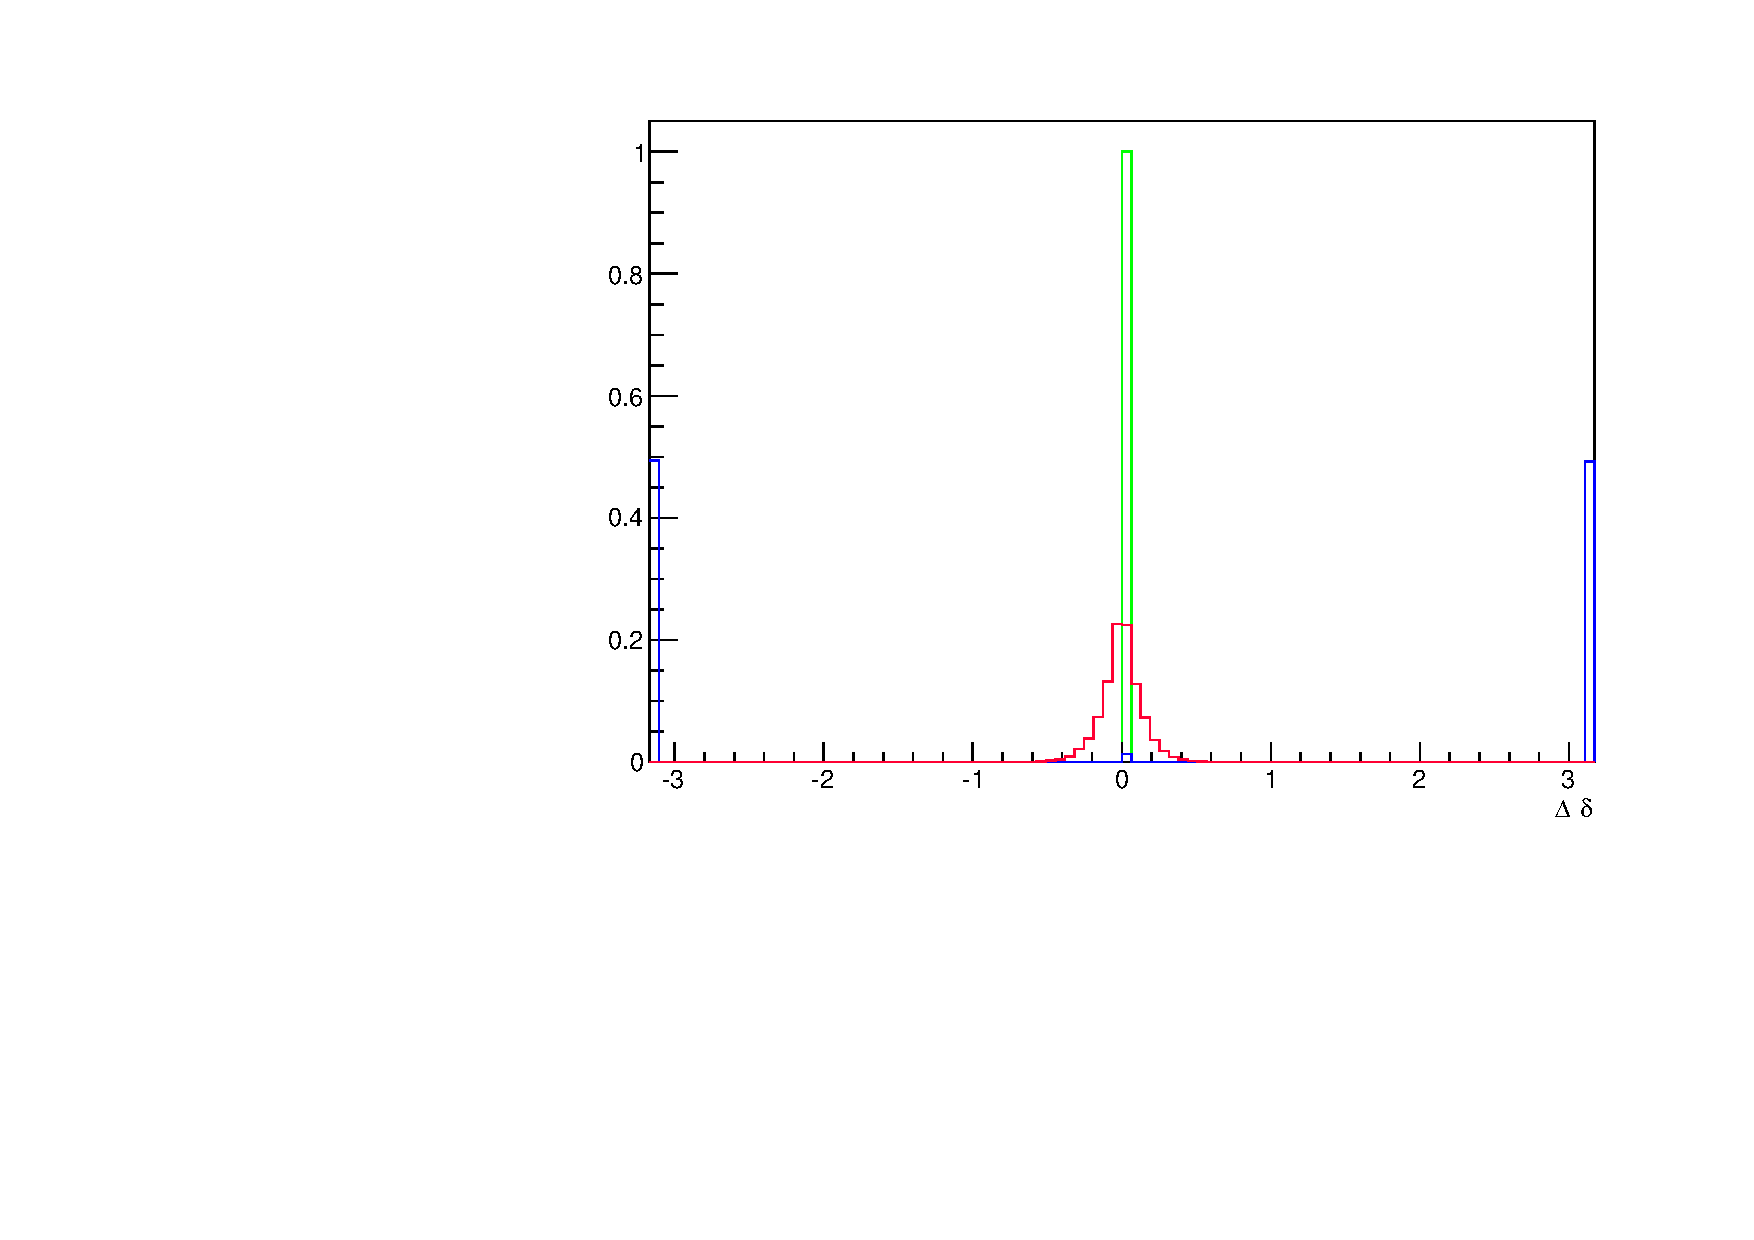
\includegraphics[width=0.49\textwidth]{phases.pdf}
  \vspace*{-0.5cm}
  \end{center}
  \caption{\textit{Distribution of the strong phase difference for the current \Dz decay amplitude (pink), and the \CP even (green) and \CP odd (blue) amplitudes constructed.}}
  \label{fig:siggen}
\end{figure}
In the course of this investigation an error in the computation of the \CP conjugate amplitude was found and immediately fixed by Jonas \footnote{More errors might have been discovered recently and shall be fixed soon.}.\\


\section{Dalitz Markov Chain Monte Carlo}
Markov Chain Monte Carlo (MCMC) is based on the Metropolis-Hasting s algorithm and is a way of generating MC events very fast. \\
The algorithm picks a first random point \textbf{p} in phasespace and adds it to the eventlist. From this first point another point \textbf{p'} is chosen according to a function $g(p \rightarrow p')$. Then an accept-reject selection on the second point is performed based on the \PDF values of both points:
\begin{enumerate}
\item if $|A(p')|^2 > |A(p)|^2$ the event described by \textbf{p'} is accepted and the algorithm begins again with \textbf{p'} as \textbf{p}.\\
\item if $|A(p')|^2 < |A(p)|^2$ a number $h$ is randomly generated between 0 and 1,\\
\begin{itemize}
\item if $h < \frac{|A(p')|^2}{|A(p)|^2}$ the event described by \textbf{p'} is accepted and the algorithm begins again with \textbf{p'} as \textbf{p}.\\
\item if $h > \frac{|A(p')|^2}{|A(p)|^2}$ the event described by \textbf{p'} is rejected, the event described by \textbf{p} is stored in the eventlist again and the algorithm begins again with \textbf{p}. \\
\end{itemize}
\end{enumerate}
Because at each iteration an event is saved the MCMC is much faster than the conservative MC algorithm that is used in the \texttt{SignalGenerator} class. Unfortunately there is a high chance of copying the exact same events which can introduce a bias.\\


\subsection{Implementation and improvement}
The MCMC has been implemented in \mint by Jeremy in a class named \texttt{DalitzMCMC} and tested to show that it reproduces the same invariant mass distributions as the conservative \texttt{SignalGenerator}.\\
\\
While the \texttt{DalitzMCMC} reproduces the correct distributions it has the disadvantage of copying the same events which biases the sample for a small number of events. In order to prevent this a huge sample of events is generated from which the desired number of events is randomly chosen. Therefore a \textbf{rejection factor} is added to the generation method which determines what percentage of events are discarded \footnote{A rejection factor of n means that one event in n will be saved.}.\\
A study is performed by generating 10\,000 events for six different rejection factors respectively. This is done using two different amplitude models. The first amplitude is the current \Dz model obtained from CLEO-c data while the second model consists of only one very narrow resonance.\\
\\
Figure \ref{fig:rep} shows the percentage of events that are exact copies of another event depending on the rejection factor. The percentage of repeated events clearly depends on the amplitude model as well as on the rejection factor. For the current \Dz decay model a rejection factor of 10\,000 should make sure that absolutely no single event is repeated twice.\\
\begin{figure}[!h]
\vspace*{-0.cm}
  \begin{center}
 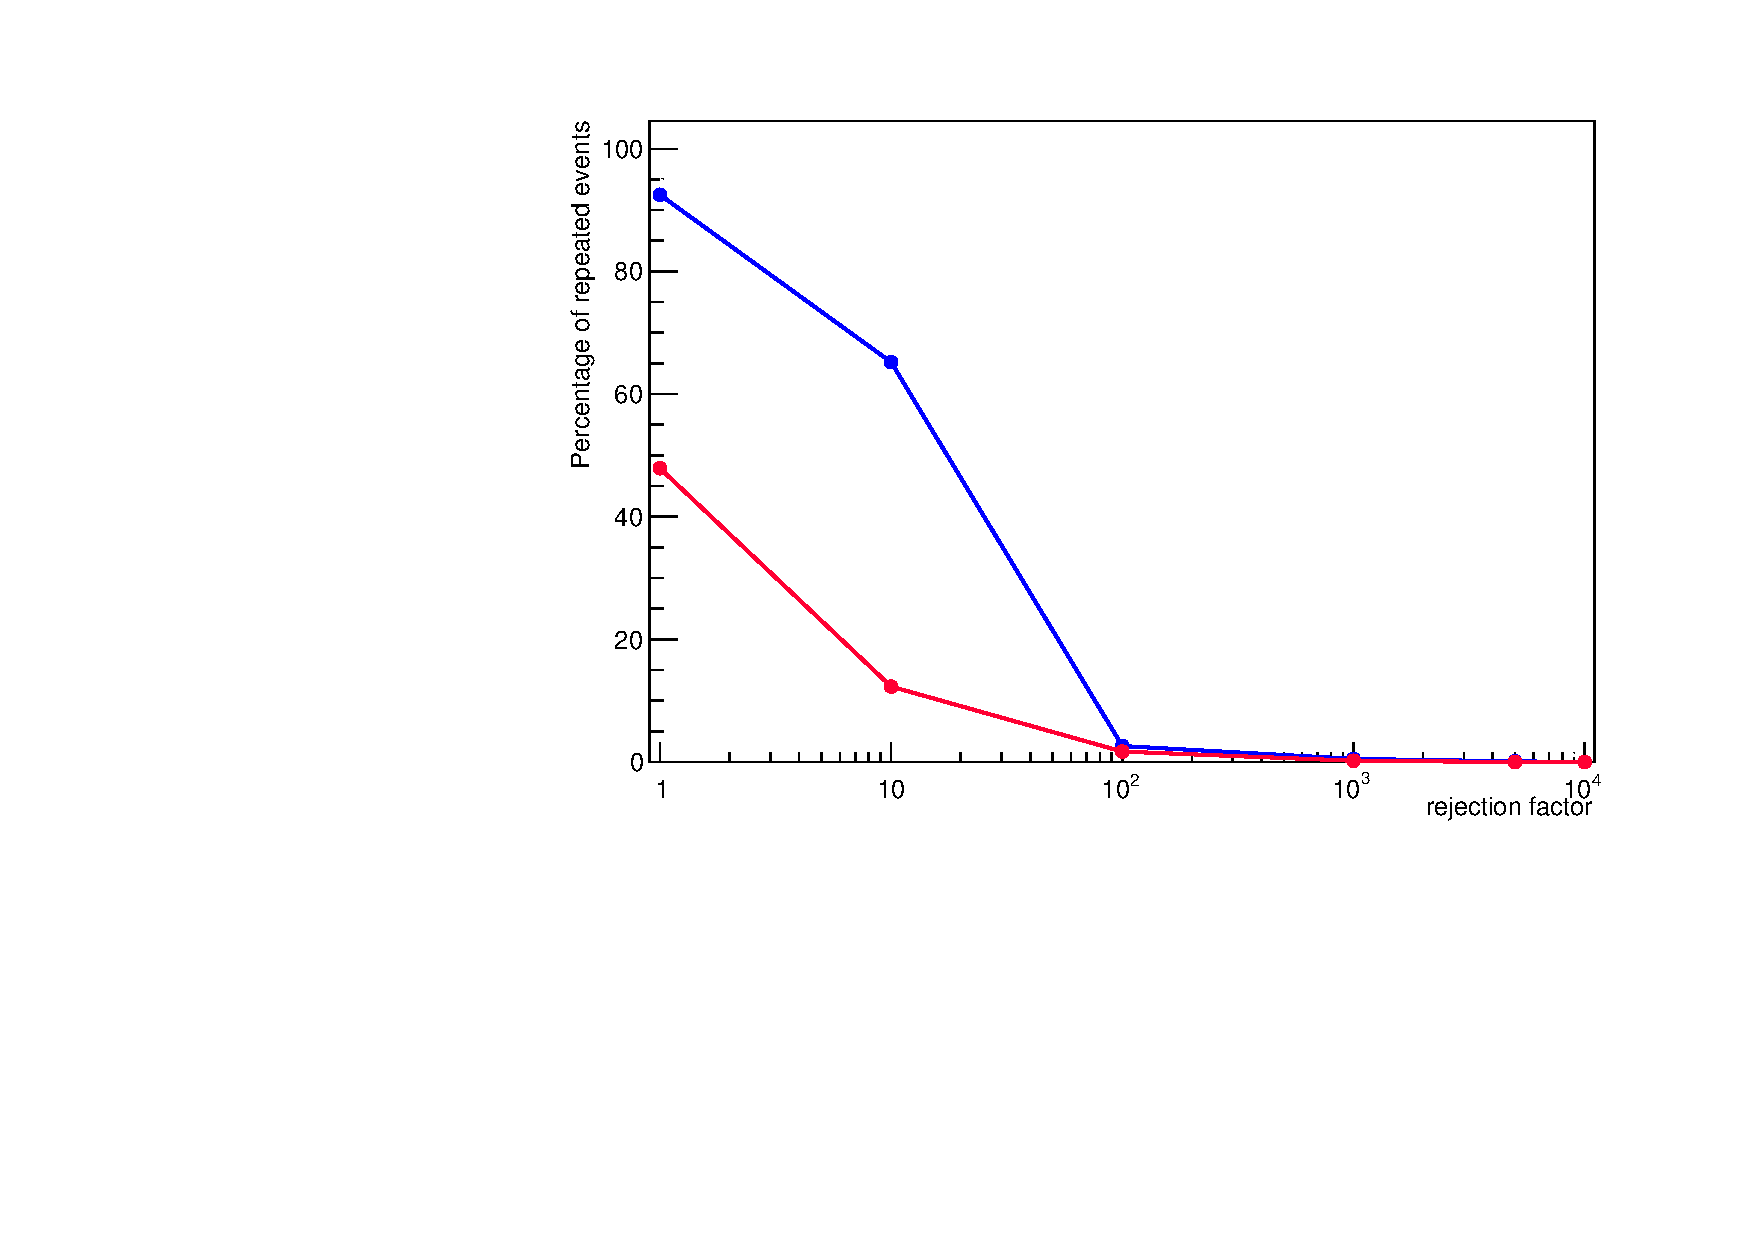
\includegraphics[width=0.49\textwidth]{repeat.pdf}
  \vspace*{-0.5cm}
  \end{center}
  \caption{\textit{Percentage of repeated events in the generation of 10\,000 \DzTo4Pi events using the \texttt{DalitzMCMC} class. The pink line represents the current \Dz amplitude model while the blue line represents the amplitude consisting of one very narrow resonance.}}
  \label{fig:rep}
\end{figure}

Figure \ref{fig:hauf} shows the frequency of which events are repeated for the six different rejection factors and the two different amplitude models. This shows that most events are repeated only once.\\
\begin{figure}[!h]
\vspace*{-0.cm}
  \begin{center}
  \subfigure{\label{fig:hauf1a}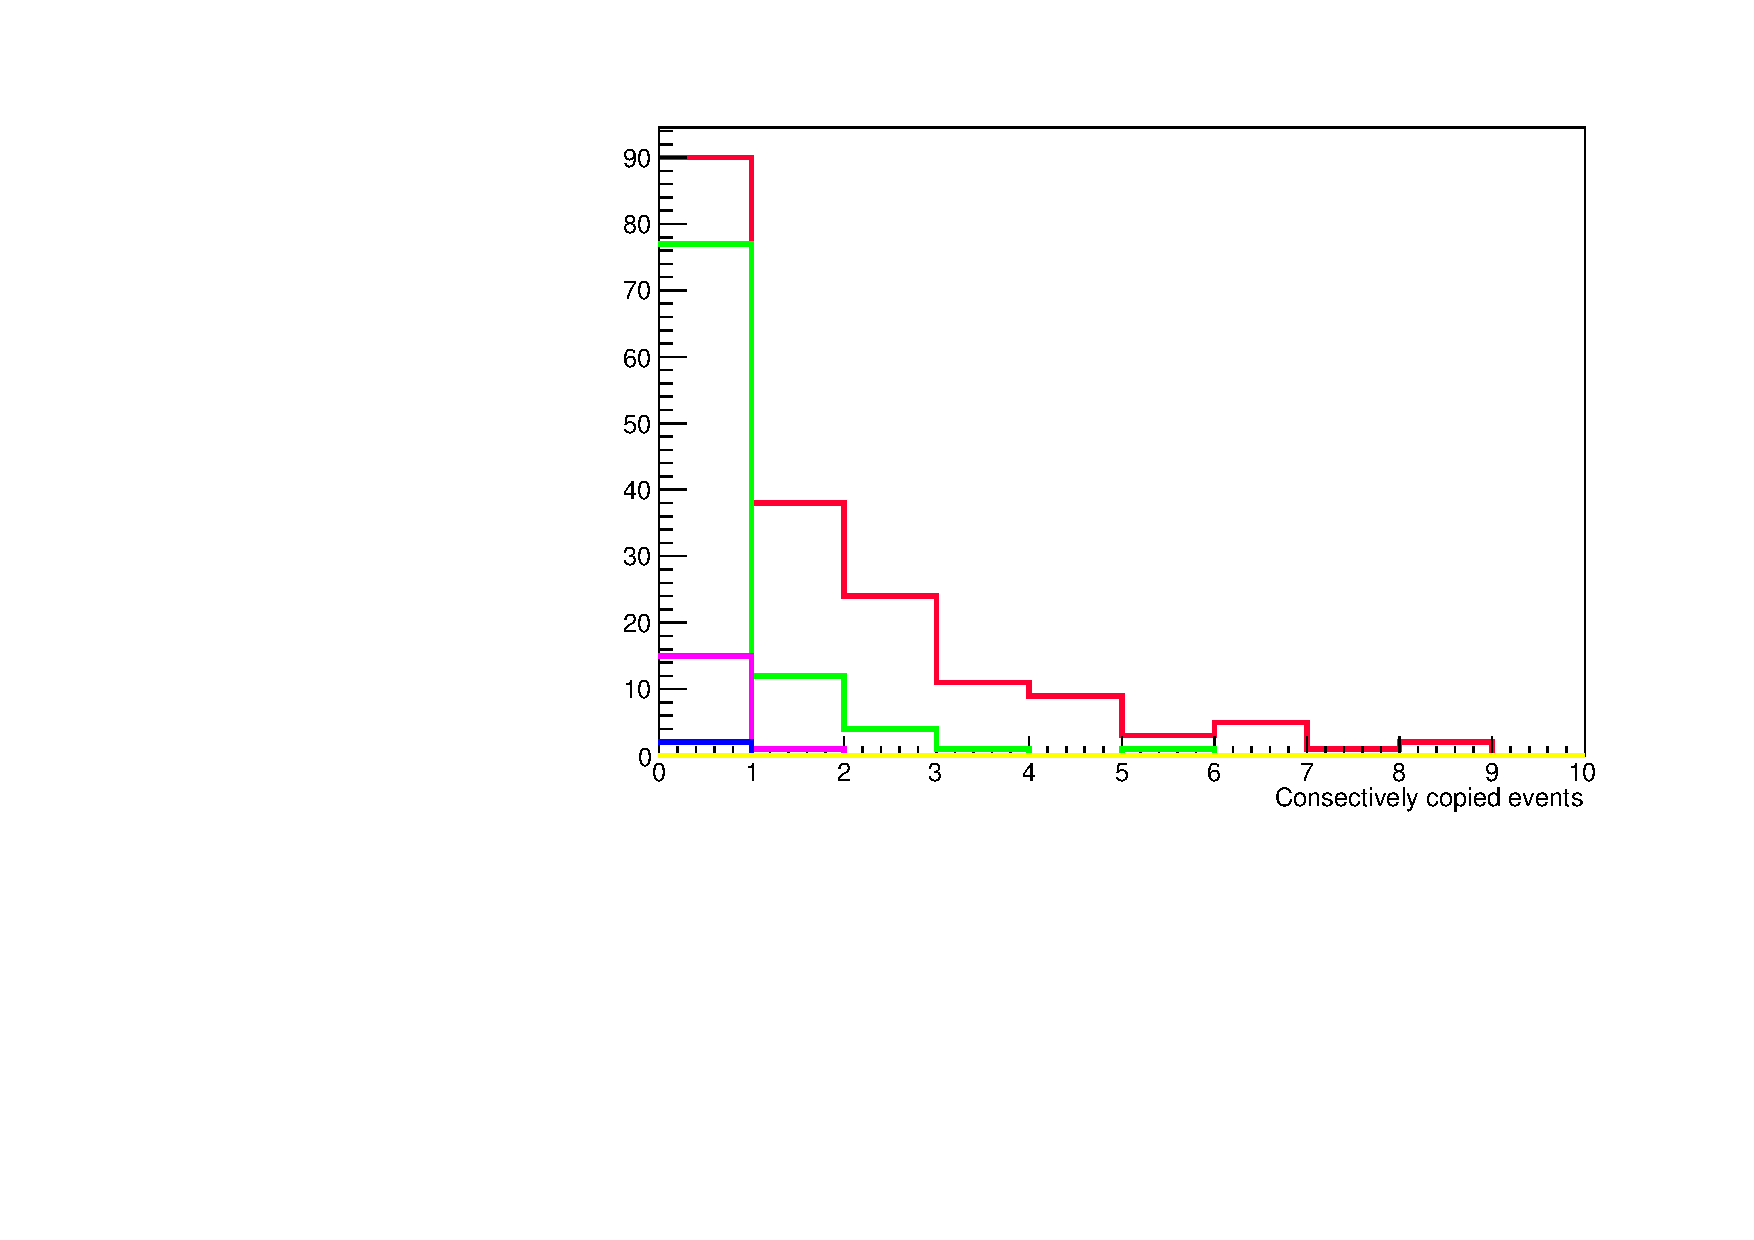
\includegraphics[width=0.49\textwidth]{haeufigkeit.pdf}}
  \subfigure{\label{fig:hauf1b}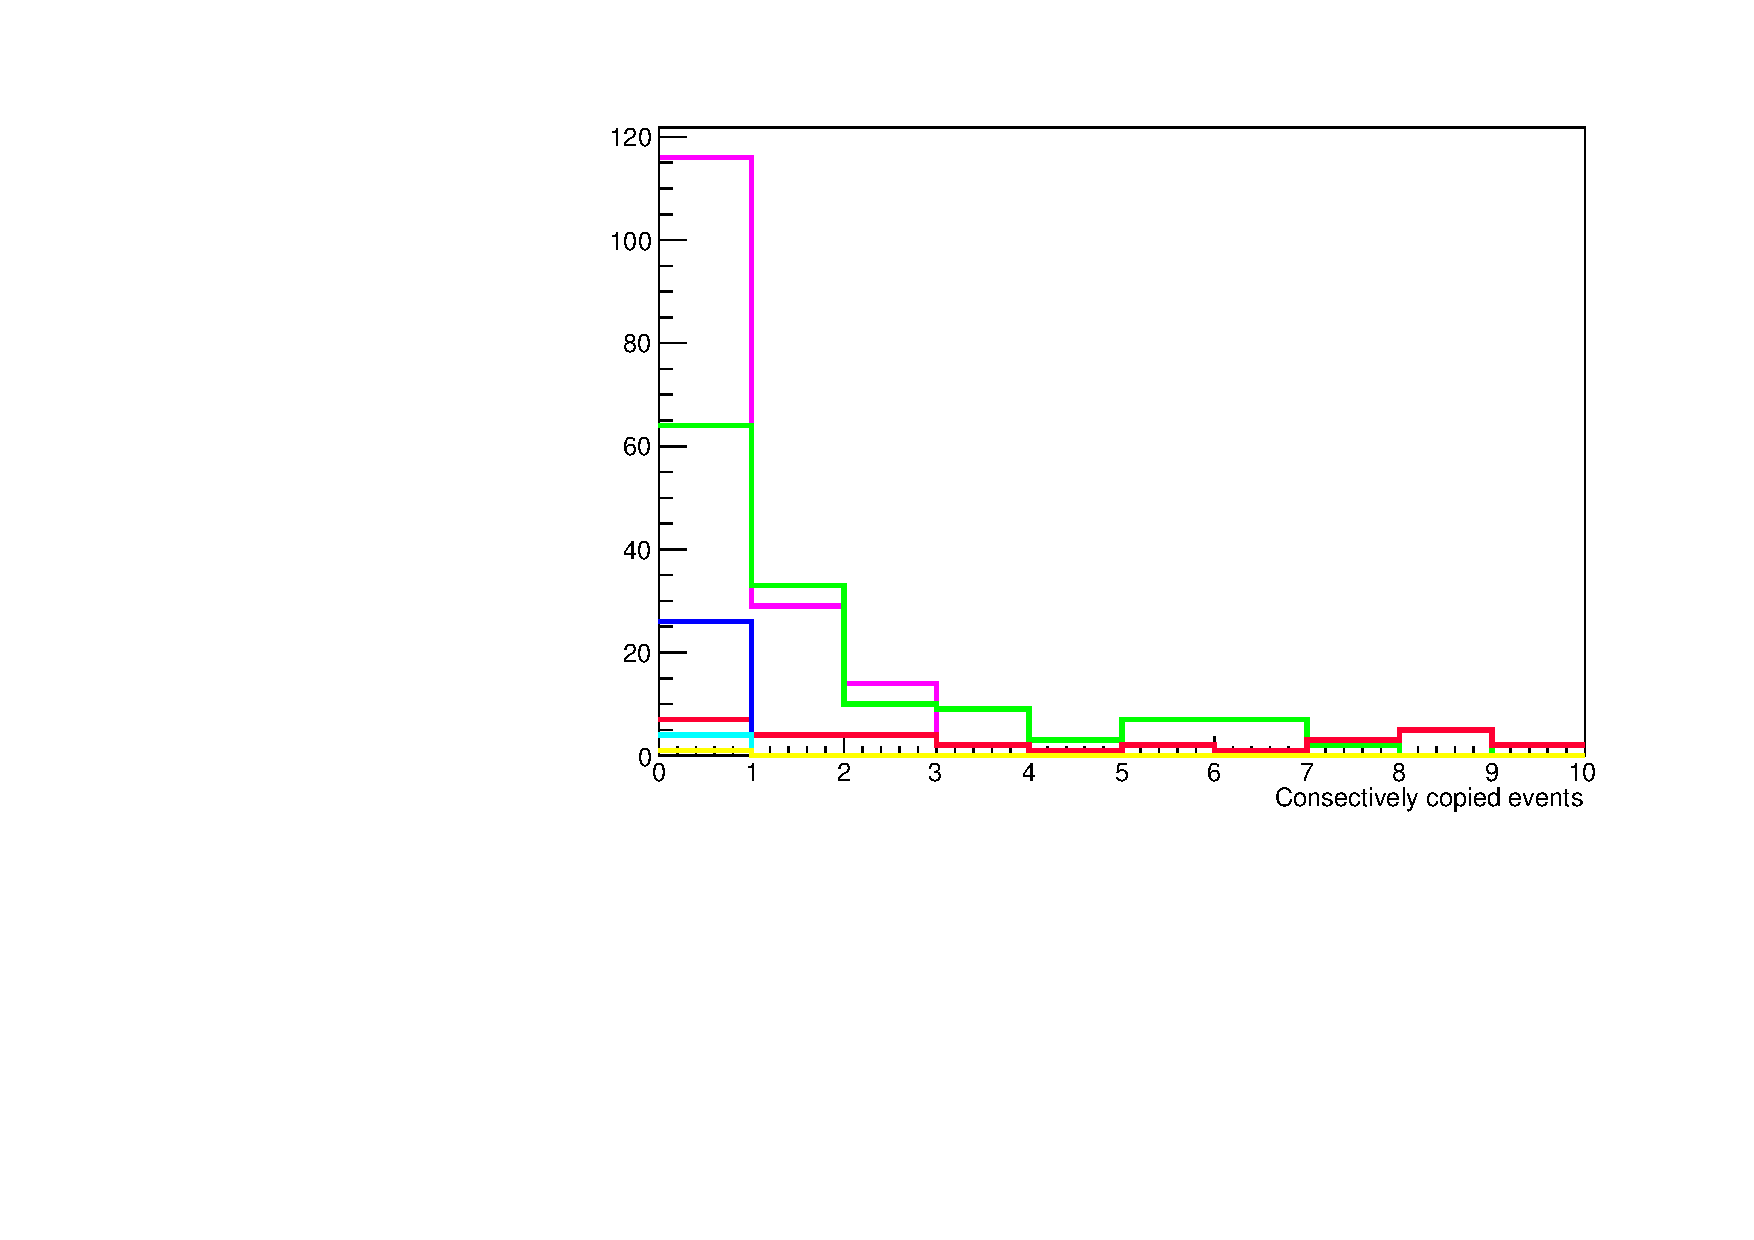
\includegraphics[width=0.48\textwidth]{haeufigkeit_a1.pdf}} 
  \vspace*{-1.0cm}
  \end{center}
  \caption{\textit{Amount of times that a certain event occurs in the sample of 10\,000 \DzTo4Pi sample generated with the \texttt{DalitzMCMC} class for the six different rejection factors: 1 (pink), 10 (green), 100 (magenta), 1000 (blue), 5000 (cyan) and 10\,000 (yellow). The left plots shows the distribution for the current \Dz amplitude model while the right plot shows the amplitude model consisting of one very narrow resonance.}}
  \label{fig:hauf}
\end{figure}


Figure \ref{fig:time} shows the time dependence of the generation of the 10\,000 events of the rejection factors. While the time depends linearly on the rejection factor, it also highly depends on the amplitude model.\\ 
Using a rejection factor of 10\,000 makes the generation slightly slower than using the \texttt{SignalGenerator} class. The indisputable advantage of the \texttt{DalitzMCMC} generator over the \texttt{SignalGenerator} will be shown in the next section.\\
\begin{figure}[!h]
\vspace*{-0.cm}
  \begin{center}
 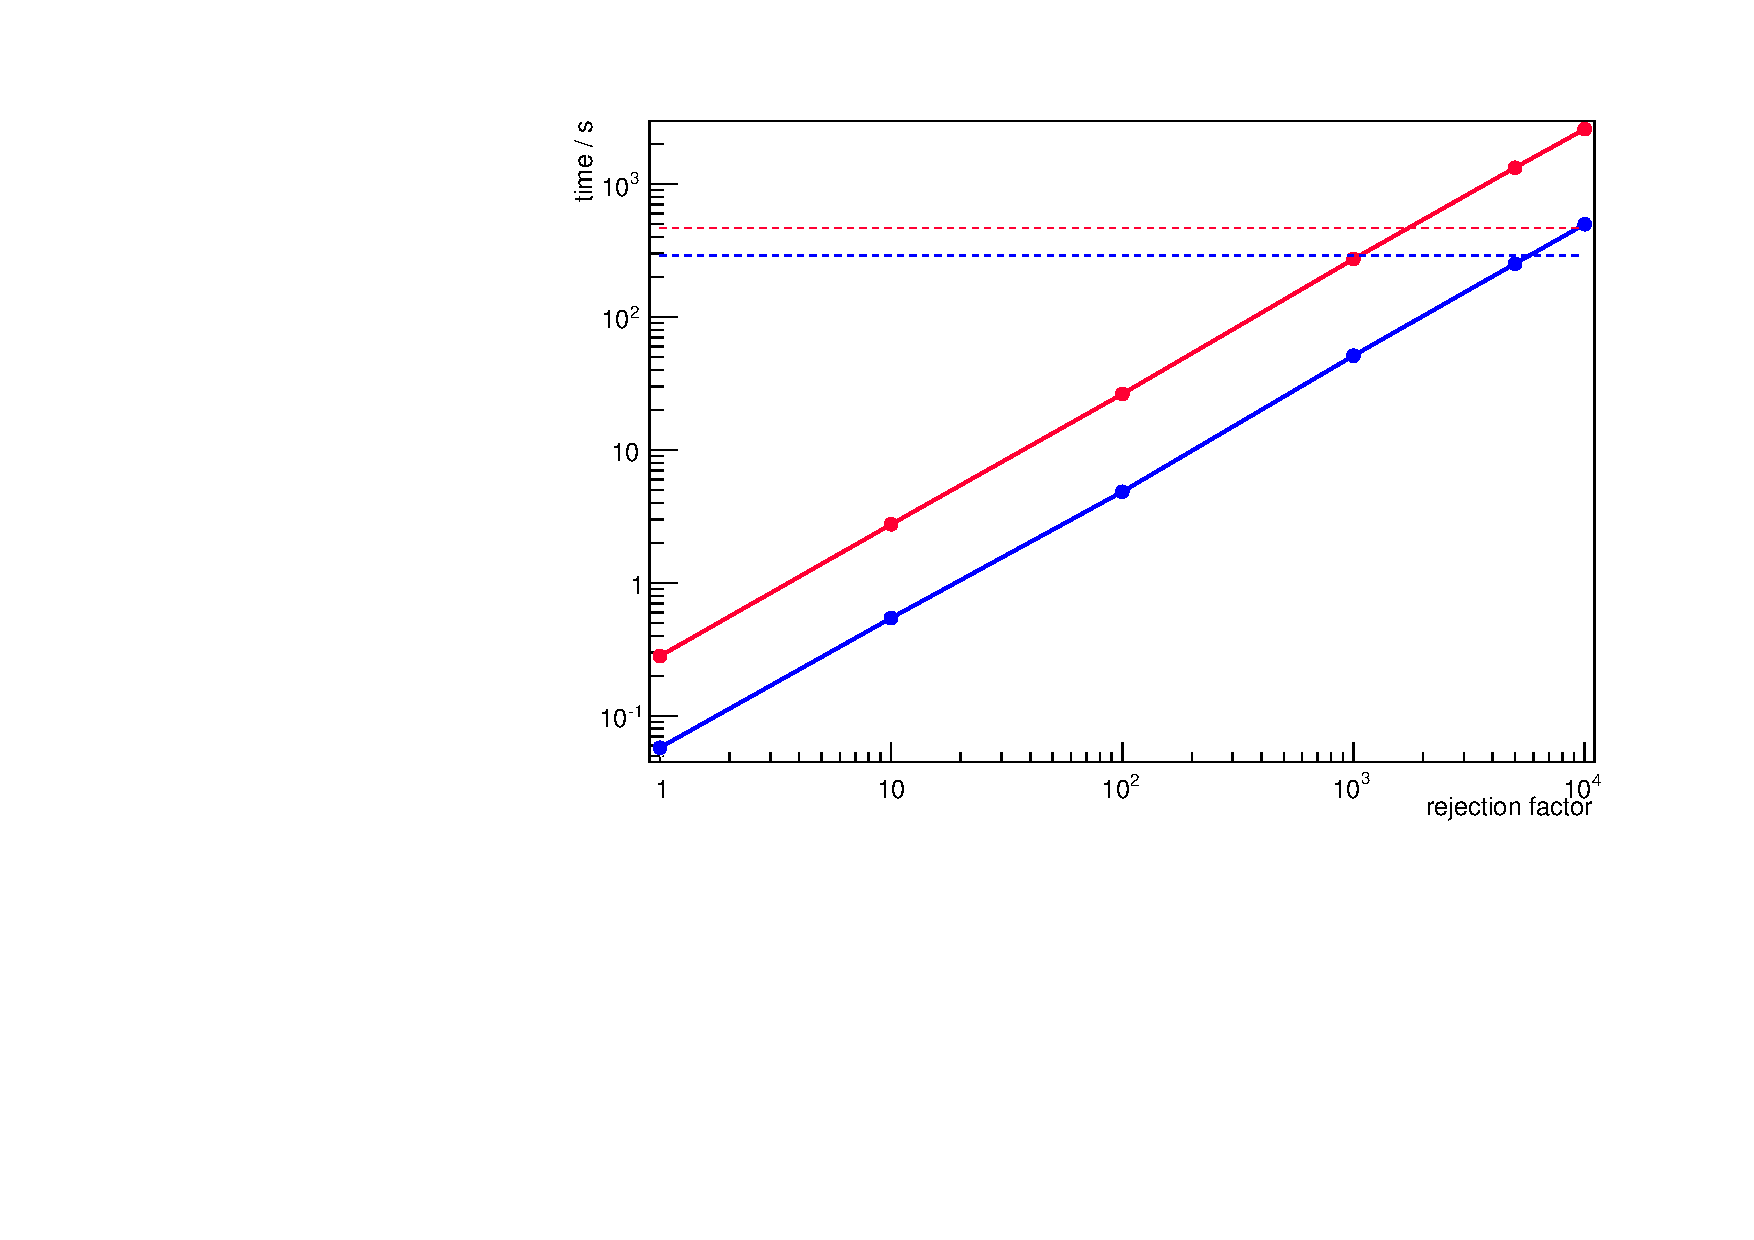
\includegraphics[width=0.49\textwidth]{timedep.pdf}
  \vspace*{-0.5cm}
  \end{center}
  \caption{\textit{Time dependence of the generation of 10\,000 \DzTo4Pi events using the \texttt{DalitzMCMC} class. The pink line represents the natural \Dz amplitude model while the blue line represents the amplitude consisting of one very narrow resonance. The dotted lines show the time values for the generation of 10\,000 events using the \texttt{SignalGenerator} class.}}
  \label{fig:time}
\end{figure}



\section{Correlated Dalitz Monte Carlo}
While \mint is a powerful tool for generating (and fitting) multibody \D decays it did not have the possibility to generate the correlated \Dz - \Dzb pairs that are needed for this analysis. Therefore a class named \texttt{DalitzMCMC\_corrPairs} was implemented that generates these events using the an adapted version of the MCMC algorithm.\\

\subsection{Implementation}
In order to generate the correlated pairs the \texttt{DalitzMCMC\_corrPairs} is given two \Dz decay amplitudes. It then generates two independent events, flat in phasespace, using the \texttt{TGenPhaseSpace} class. These events are then evaluated after the MCMC algorithm to obey the \PDF for correlated pairs
\begin{equation}
A(f_{1} f_{2}) = \frac{A(\Dz \rightarrow f_1) A(\Dzb \rightarrow f_2) - A(\Dz \rightarrow f_2) A(\Dzb \rightarrow f_1)}{\sqrt{2}}
\end{equation} 
where the minus sign originates from the spin-parity factor of the \psiprpr.\\
The implementation of all classes and methods was kept as similar to the according classes and methods for the \texttt{SignalGenerator} and the \texttt{DalitzMCMC} as possible.\\

\subsection{Testing}
The DalitzMCMC corrPairs is tested using the fact that if the flavour / \CP value of one final state is known, the other one is fixed to its opposite.\\
Ten thousand correlated pairs were generated for two different sets of amplitudes and final states.\\

\subsubsection{\CP eigenstates}
In order to test the correlation behaviour for \CP eigenstates the \D final states are chosen to be $4\pion$ on one side and $\KS \pip \pim$ on the other. The implemented decay amplitudes and their \CP value are listed in Table \ref{tab:corr1}.\\
\begin{table}[!h]
\begin{center}
\begin{tabular}{l|c|c}
final state & amplitude & \CP value   \\
\hline
$4 \pion$ & $\Dz \rightarrow \rho^0(770)(\rightarrow \pip \pim) \rho^0(770)(\rightarrow \pip \pim) $ P-wave  & even \\
$4 \pion$ & $\Dz \rightarrow f_0(980)(\rightarrow \pip \pim) \rho^0(980)(\rightarrow \pip \pim) $  & odd \\
\hline
$\KS \pip \pim$ & $\Dz \rightarrow \rho^0(770)(\rightarrow \pip \pim) \KS $  & even \\
\end{tabular}
\end{center}
\vspace*{-0.5cm}
\caption{\textit{Decay amplitudes that make up the amplitude model for the two different final states and their \CP value.}}
\label{tab:corr1}
\end{table}

\begin{figure}[!h]
\vspace*{-0.cm}
  \begin{center}
  \subfigure{\label{fig:corr1a}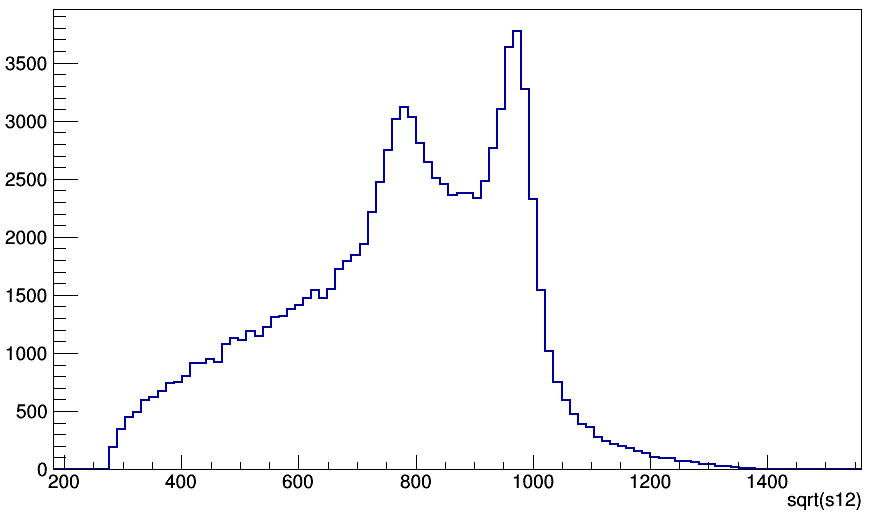
\includegraphics[width=0.49\textwidth]{Corr1a.png}}
  \subfigure{\label{fig:corr1b}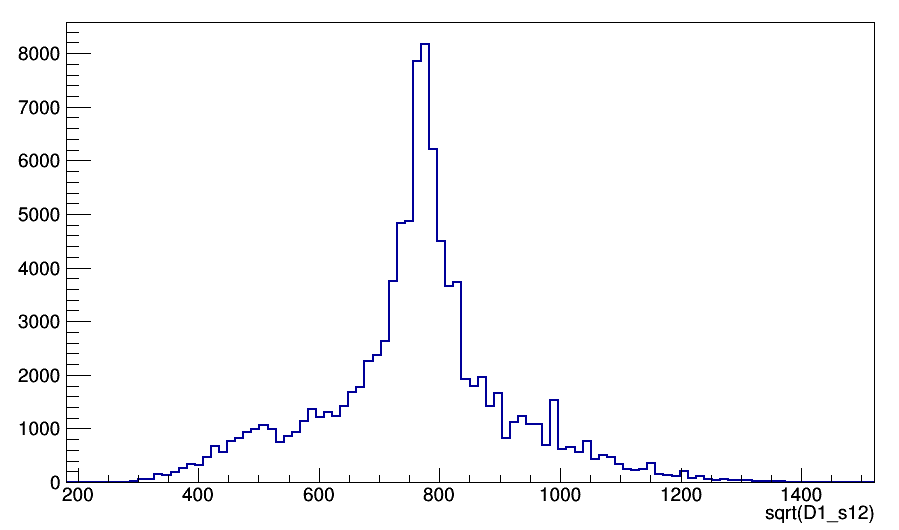
\includegraphics[width=0.48\textwidth]{Corr1b.png}} 
  \vspace*{-1.0cm}
  \end{center}
  \caption{\textit{Invariant mass m(\pip \pim) distribution of two opposite sign pions from the \DTo4Pi decays generated with \mint 's \texttt{DalitzMCMC} (left) and the \texttt{DalitzMCMC\_corrPairs} with the $\D \rightarrow \KS \pip \pim$ decay listed in Table \ref{tab:corr1} on the other side (right). The widths of the resonances were altered in the simulation to make the peaks from the resonances distinguishable.}}
  \label{fig:corr1}
\end{figure}

Figure \ref{fig:corr1} shows the invariant mass distribution of two opposite sign pions from the \DTo4Pi decays for singly generated events and correlated events. It is obvious that the peak from the $f_0$ does not appear in the correlated events. This is due to the fact that the $f_0$ resonance comes from a \CP even amplitude which is forbidden by setting the amplitude of the other side \D meson to \CP even only.\\

\subsubsection{Flavour eigenstates}
In order to test the correlation behaviour for the flavour specific states the \D final states are chosen to be $4\pion$ and $\KS \pip \pim$ again but with the decay amplitudes chosen to be a single flavour specific state for both decays as listed in Table \ref{tab:corr2}.\\
\begin{table}[!h]
\begin{center}
\begin{tabular}{l|c}
final state & flavour specific amplitude   \\
\hline
$4 \pion$ & $\Dz \rightarrow a_1^+(1260)\rightarrow (\rightarrow \pip \pip \pim) \pim $ \\
\hline
$\KS \pip \pim$ & $\Dz \rightarrow \Kstarm(\rightarrow \KS \pim) \pip $   \\
\end{tabular}
\end{center}
\vspace*{-0.5cm}
\caption{\textit{Flavour specific decay amplitudes for the two different final states.}}
\label{tab:corr2}
\end{table}
Making a cut on the invariant mass of the \KS \pim pair around the \Kstarm mass fixes most of the $\D \rightarrow \KS \pip \pim$ decays to coming from a \Dz which means that the $\D \rightarrow 4 \pion$ events must come from a \Dzb meson and the $a_1$ resonance should be negative (therefore not visible in the $m(\pip \pip \pim)$ distribution). As can be seen in Figure \ref{fig:corr2} this is the case.\\

\begin{figure}[!h]
\vspace*{-0.cm}
  \begin{center}
 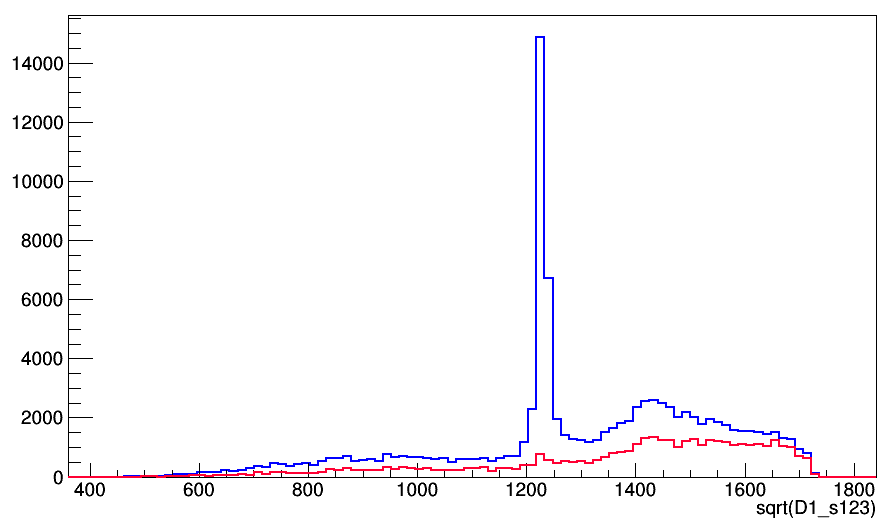
\includegraphics[width=0.49\textwidth]{a1peak.png}
  \vspace*{-0.5cm}
  \end{center}
  \caption{\textit{Invariant mass m(\pip \pip \pim) distribution of three pions from the \DTo4Pi decays generated with \mint \texttt{DalitzMCMC\_corrPairs} class with  the $\D \rightarrow \KS \pip \pim$ decay listed in Table \ref{tab:corr2}. The width of the resonance was altered in the simulation to make the peaks from the resonances distinguishable.}}
  \label{fig:corr2}
\end{figure}

\section{Future work}
The work for the next year includes the following steps
\begin{itemize}
\item MC study of $c_i$ and $s_i$ measurement
\item extract the data from CLEO-c: \DTo4Pi events vs. several flavour / \CP tags, \DTo4Pi vs. \DTo4Pi and \DTo4Pi vs $\D \rightarrow \KS \pip \pim$
\item decide if the phase-binning is the most convenient one
\item measure $c_i$ and $s_i$ and compare to model prediction
\item publish Jack's \DzTo4Pi model and the $c_i$ and $s_i$ measurement
\end{itemize}